\subsubsection{Ring code}
The ring code's graph essentially simply loops around at the repetition
code's single-edged ancilla nodes via an additional ancilla. 
It's edge matrix where the \emph{n}th row
represents which data qubit is connected to the nth ancilla
qubit is the following:
\begin{equation}
    M_{pc3} = \left(
        \begin{array}{ccc}
            1 & 1 & 0\\
            0 & 1 & 1\\
            1 & 0 & 1\\
        \end{array}
        \right)
\end{equation}

\begin{figure}[h!]
	\begin{center}
	\captionsetup{justification=centering,margin=2cm}
	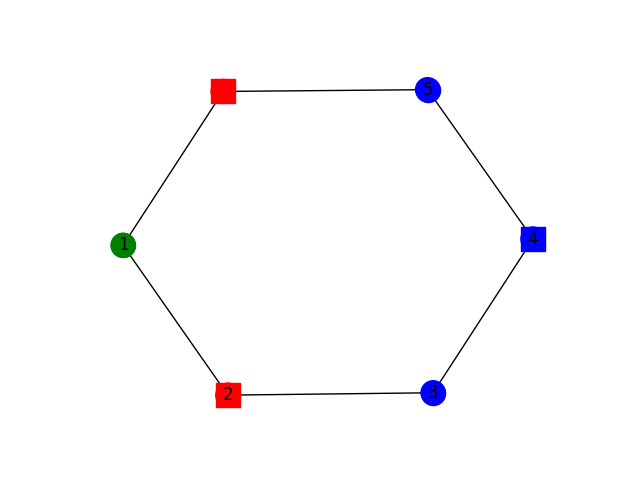
\includegraphics[scale=0.25]{./img/figures/ring_3_graph.png}\\
	\caption{Graph for [[3,1,$\frac{1}{2}$]] ring code with error on node
    1 marked in green and resulting syndrome marked in red.
    Squares represent ancilla qubits and circles represent data qubits.}
        
	\label{fig: ring_graph}
	\end{center}
\end{figure}

